\documentclass{article}
% Chinese
% \documentclass[UTF8, nofonts, mathptmx, 12pt, onecolumn]{article}
% \usepackage{xeCJK}
% \setCJKmainfont{SimSun}
\usepackage{amsmath}
\usepackage{amsfonts}
\usepackage{amssymb}
\usepackage{wasysym}
% \usepackage{ctex}
\usepackage{graphicx}
\usepackage{float}
\usepackage{geometry}
\geometry{a4paper,scale=0.8}
\usepackage{caption}
\usepackage{subcaption}
% \newcommand{\oiint}{\mathop{{\int\!\!\!\!\!\int}\mkern-21mu \bigcirc} {}}
\newcommand*{\dif}{\mathop{}\!\mathrm{d}}
\newcommand*{\md}{\mathop{}\!\mathrm{d}}
\newcommand*{\me}{\mathrm{e}}

% \usepackage{parskip}
% \setlength{\parindent}{0cm}

\usepackage{bm}
\let\Oldmathbf\mathbf
\renewcommand{\mathbf}[1]{\boldsymbol{\Oldmathbf{#1}}}
\let\eqnarray\align

\author{Xiping Hu}
\usepackage{authblk}
\author{Xiping Hu}
\affil{https://hxp.plus/}
\title{Homework for Chapter 6}

\begin{document}
\maketitle

\begin{figure}[H]
  \centering
  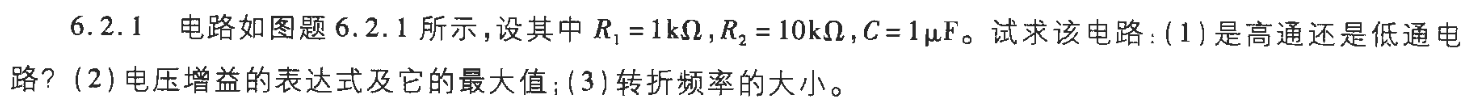
\includegraphics[width=\linewidth]{figures/Problem621}
  \label{fig:}
\end{figure}

\begin{figure}[H]
  \centering
  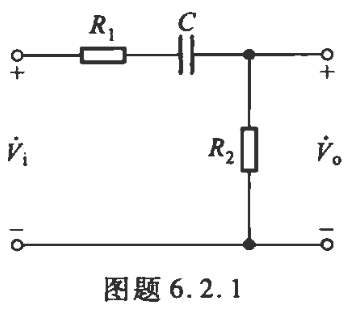
\includegraphics[width=0.4\linewidth]{figures/Problem6211}
  \label{fig:}
\end{figure}

The circuit is a High-pass filter, since the impedance of capacitor is represented as

\begin{equation*}
  \begin{aligned}
    R_C = \dfrac{1}{s C} \quad\quad s = j \omega 
  \end{aligned}
\end{equation*}

The gain of this circuit is represented as

\begin{equation*}
  \begin{aligned}
    \dfrac{V_o}{V_i}
  \end{aligned}
\end{equation*}

Whereas

\begin{equation*}
  \begin{aligned}
    V_o = \dfrac{R_2}{R_1 + \dfrac{1}{sC} + R_2 } V_i = \dfrac{R_2}{R_1 + R_2} \dfrac{s}{s + \dfrac{1}{C \left( R_1 + R_2 \right)} }   
  \end{aligned}
\end{equation*}

So that the corner frequency is

\begin{equation*}
  \begin{aligned}
    f_0 = \dfrac{1}{2 \pi C \left( R_1 + R_2 \right)} \approx 14.5 \  \mathrm{Hz}
  \end{aligned}
\end{equation*}

The gain of the circuit is

\begin{equation*}
  \begin{aligned}
    \dfrac{V_o}{V_i} = \dfrac{R_2}{R_2 + R_1} \dfrac{s}{s + \omega_0} \quad\quad \omega_0 = \dfrac{1}{C \left( R_1 + R_2 \right)}   
  \end{aligned}
\end{equation*}

The maximum gain is

\begin{equation*}
  \begin{aligned}
    \left. \dfrac{V_o}{V_i}  \right|_{max} = \dfrac{R_2}{R_2 + R_1} \approx 0.909
  \end{aligned}
\end{equation*}

\end{document}